%\documentclass[times, 10pt, twocolumn]{article}
%\documentclass[conference,final]{IEEEtran}
     
\documentclass{rspublic}   

%-------------------------------------------------------------------------
%take the % away on next line to produce the final camera-ready version
%\pagestyle{empty}

\usepackage[utf8]{inputenc}
%\usepackage{graphicx}
\usepackage{url}
\usepackage{float}
\usepackage{times}
\usepackage{multirow}
\usepackage{listings}
\usepackage{times}
\usepackage{paralist}
\usepackage{wrapfig}
\usepackage[small,it]{caption}
\usepackage{multirow}
\usepackage{ifpdf}
\usepackage{subfig} 
\usepackage[pdftex]{graphicx}
%\usepackage{harvard}
%\usepackage{pdfsync}                    
%\usepackage{subfigure}

%Bibliography     
\usepackage{natbib}                

\usepackage{listings}
\usepackage{keyval}
\usepackage{color}
\definecolor{listinggray}{gray}{0.95}
\definecolor{darkgray}{gray}{0.7}
\definecolor{commentgreen}{rgb}{0, 0.4, 0}
\definecolor{darkblue}{rgb}{0, 0, 0.4}
\definecolor{middleblue}{rgb}{0, 0, 0.7}
\definecolor{darkred}{rgb}{0.4, 0, 0}
\definecolor{brown}{rgb}{0.5, 0.5, 0}

\lstdefinestyle{myListing}{
  frame=single,   
  backgroundcolor=\color{listinggray},  
  %float=t,
  language=C,       
  basicstyle=\ttfamily \footnotesize,
  breakautoindent=true,
  breaklines=true
  tabsize=2,
  captionpos=b,  
  aboveskip=0em,
  %numbers=left, 
  %numberstyle=\tiny
}      

\lstdefinestyle{myPythonListing}{
  frame=single,   
  backgroundcolor=\color{listinggray},  
  %float=t,
  language=Python,       
  basicstyle=\ttfamily \footnotesize,
  breakautoindent=true,
  breaklines=true
  tabsize=2,
  captionpos=b,  
  %numbers=left, 
  %numberstyle=\tiny
}

\title[Understanding Performance Implications of Distributed Filesystems
in a Data-Intensive Application]{Understanding Performance Implications
of Distributed Filesystems in a Data-Intensive Application}

\author[Miceli, Miceli, Rodriguez-Milla, Jha]{
 Christopher Miceli$^{1}$, Michael Miceli$^{1}$, Bety Rodriguez-Milla$^{1}$, Shantenu Jha$^{1,2,*}$
 \small{\emph{$^{1}$Center for Computation \& Technology, Louisiana State University, USA}}
 \small{\emph{$^{2}$Department of Computer Science, Louisiana State University, USA}}
 {\footnotesize {\hspace{0.0 in} $^*$Corresponding Author sjha@cct.lsu.edu}}
}

%\date{}

\def\acknowledgementname{Acknowledgements}
\newenvironment{acknowledgement}%
{\section*{\acknowledgementname}%
\parindent=0pt%
}

\newif\ifdraft
\drafttrue
\ifdraft
\newcommand{\fixme}[1]{ { \bf{ ***FIXME: #1 }} }
\newcommand{\jhanote}[1]{ {\textcolor{red} { ***Jha: #1 }}}
\newcommand{\micnote}[1]{ {\textcolor{blue} { ***Michael: #1 }}}
\else
\newcommand{\jhanote}[1]{}
\newcommand{\micnote}[1]{}
\newcommand{\fixme}[1]{}
\fi

\begin{document}
\maketitle

\micnote{This can't be more than 200 words. The summary should be
concise and informative. It should be complete by itself, and must not
contain references or unexplained abbreviations. It should not only
indicate the general scope of the article but also state the main
results and conclusions. Please note that footnotes are not used.}

\begin{abstract}{data-intensive computing, distributed computing, cloud
computing, grid computing} Grids and, more recently, Clouds and
Cloud-like infrastructure are capable of supporting large problems.
While the capability of these systems is great, unique performance
issues appear as data-sets get extremely large, such as Google's 20
petabytes of data processed per day~\citep{google}, and trends show
continuing growth. Against this backdrop, it has become ever more
important that a distributed application developer take precautions when
placing, scheduling and managing such large volumes of data, or to state
the obvious, performance could be adversely affected greatly. As the
volume of data, and especially distributed data increases, scalable
placement and management techniques are required.  Distributed
File-Systems (DFS) simplify the management of distributed data, for
example, providing a single access protocol and a common name-space.
With the advent of several stable Open Source DFS projects (motivated in
part, by developments in Cloud Computing), these can be deployed without
explicit vendor support and are now thus, potentially useful and
effective tools to consider for data-intensive scientific applications.
DFS typically handle replication and distribution of files across
multiple machines internally and although this abstraction simplifies
the management of data, contrasted with explicit distributed aware
placement, there are potential performance trade-offs, in that the user
can no longer control data placement to optimise performance, and
possibly has performance implications.  The most common parameters
determining the performance of using DFS are the (i) number of replicas
of each data/file, (ii) number of servers. The aim of this paper is to
understand the performance trade-offs of a DFS compared to ``regular''
distribution and placement techniques, and how sensitive the performance
is in the context of a real data-intensive distributed applications.\end{abstract}

\section{Introduction} When working with distributed systems and large
data-sets together, determining whether to move input data to the
computational resource, or the computational workload to the input data
becomes very important. Frequently, there is more than one copy of the
input data for fault-tolerance reasons, then the added issue of deciding
between the two or more replicas becomes relevant. While DFS remove the
responsibility of replica management, the abstraction often makes
determining where in the DFS the data is being stored difficult, and
thus relying on the DFS protocol and internal algorithms to perform
well. Despite this, the DFS replication may alleviate these issues by
placing replicas in locations where computational resources reside.

%There are at least two types of data-intensive applications: the first
%where the actual data generated is large; the second type is where the
%data generated is small, but the volume of data on which computation
%occurs is very large. The application we used, has relatively small
%input and relatively small output, but the manner of processing causes
%many data reads. This type of application can be classified as having a
%large data throughput.  \jhanote{Can you elaborate on different types
%of data-intensive applications?  What kind is an ImageMagic based
%application?}

In this paper, we use an application based upon a Grid-enabled All-Pair
abstraction~\citep{Interop, AllPairs}. This application applies an
operation on the input data-set such that every possible pair in the set
is input to the operation. The operation we chose is to compare images
using ImageMagick and the result is a numerical value between 0 and
1~\citep{imagemagick}. It has large input $O$(GB) and relatively small
output $O$(KB). However, the manner of processing causes many
data reads. This type of application can be classified as having a
large data throughput. To handle seamlessly the
DFS and gridftp based data stores, the application uses the Simple API for Grid
Applications (SAGA) ~\citep{saga_web}. This allows the same exact
application to be used for all of our experiments. The result of this
application is stored in a matrix. The application spawns distributed
jobs to run sets of these pairs.  The problem becomes determining which
pairs to put into a set, and with which distributed resource to run that
set. If transferring data to the job takes too long, we spend more time
on data management than computation. There may be a resource capable of
the work that may be slower than others, but network-close (able to be
accessed in a relatively quick manner via the network supporting the
distributed system) enough to the data to make up for its lack of
computational ability. In our experiments, we used CloudStore (formerly
KFS), an open-source high performance distributed filesystem that builds
upon ideas from Google's distributed filesystem GFS ~\citep{kfs_web}.
CloudStore was chosen for its high performance focus, C++
implementation, and its source code availability.

\section{SAGA}
\section{AllPairs}
\section{KFS}
\section{GridFTP}
\section{Experiments} We developed three types of experiments
in order to compare distributed filesystems with manual file management.
Does a distributed filesystem grow more slowly than manual placement of
data?  When manually handling data, what are the advantages of being able
to move work to data to the work?  We focused on three variables to 
measure data:  degree of distribution, data dependency, and workload.

\subsection{Experiment I} In the first experiment, we run the SAGA-based
All-Pairs application on up to 4 machines on a Grid (LONI), without any
specific data placement strategy; also, no replication or
fault-tolerance takes place. The application sequentially assigns data
to the first available computational resource, and all data is accessed
via the gridftp protocol.
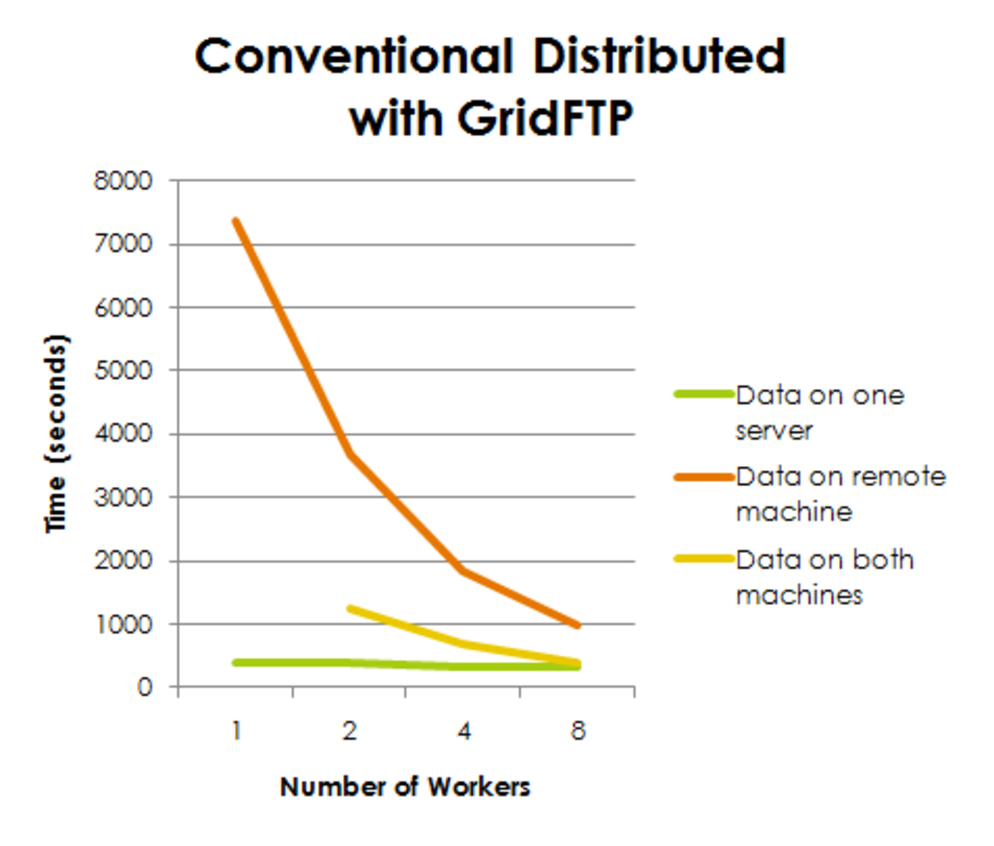
\includegraphics[width=\textwidth]{ConventionalDistributed.pdf}
\subsection{Experiment II} The second experiment is similar to the
first, except the All-Pairs application takes the data's location into
consideration when determining whether or not to assign a certain
data-set to an idle job. Inspired by earlier work~\citep{netperf}, this
version of the application performs an extra step that determines the
performance of the network by pinging hosts that may be involved, and
utilises this information when deciding which data-set to assign to a
job requesting work. Though not very sophisticated, it is a
first-approximation to performance model aware data-placement strategy.
If there is an unprocessed data-set collocated or network-close with the
job, then the assignment of that worker to that data-set would have
benefits. If there is no unprocessed data-set network-close to the job,
still we assign data that may be network-far, in case the network-close
job failed or there is no available jobs network-close to the data-set.
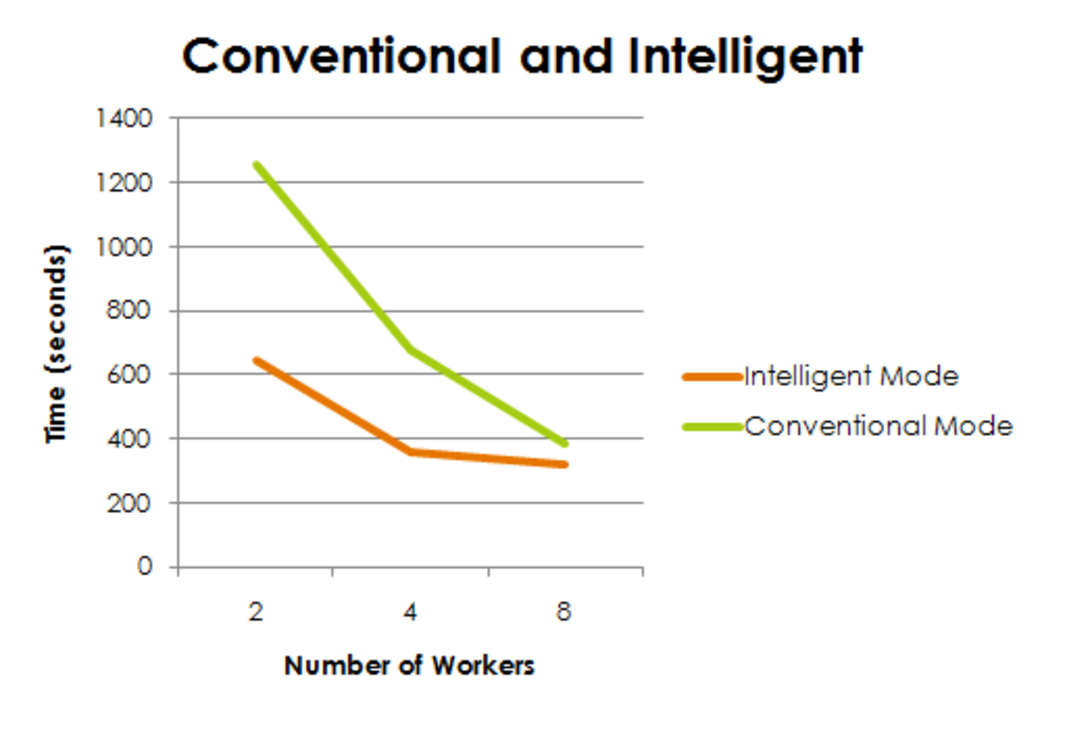
\includegraphics[width=\textwidth]{ConventionalIntelligent.pdf}
\subsection{Experiment III} The third experiment provides information
into DFSs performance in handling data locality issues. The same
All-Pairs application as in Experiments 1 and 2 is used, except all data
is stored in the distributed filesystem CloudStore with varying
replication factors, starting from two (each file is guaranteed to be
replicated at least twice). All read and writes also utilise the
distributed filesystem.  Since the performance of this test is dependent
on where the DFS stores data relative to the computational resources of
the system, we place block-servers on every machine that may be capable
of performing work.  This places all responsibility on the DFS in
determining where to place data.
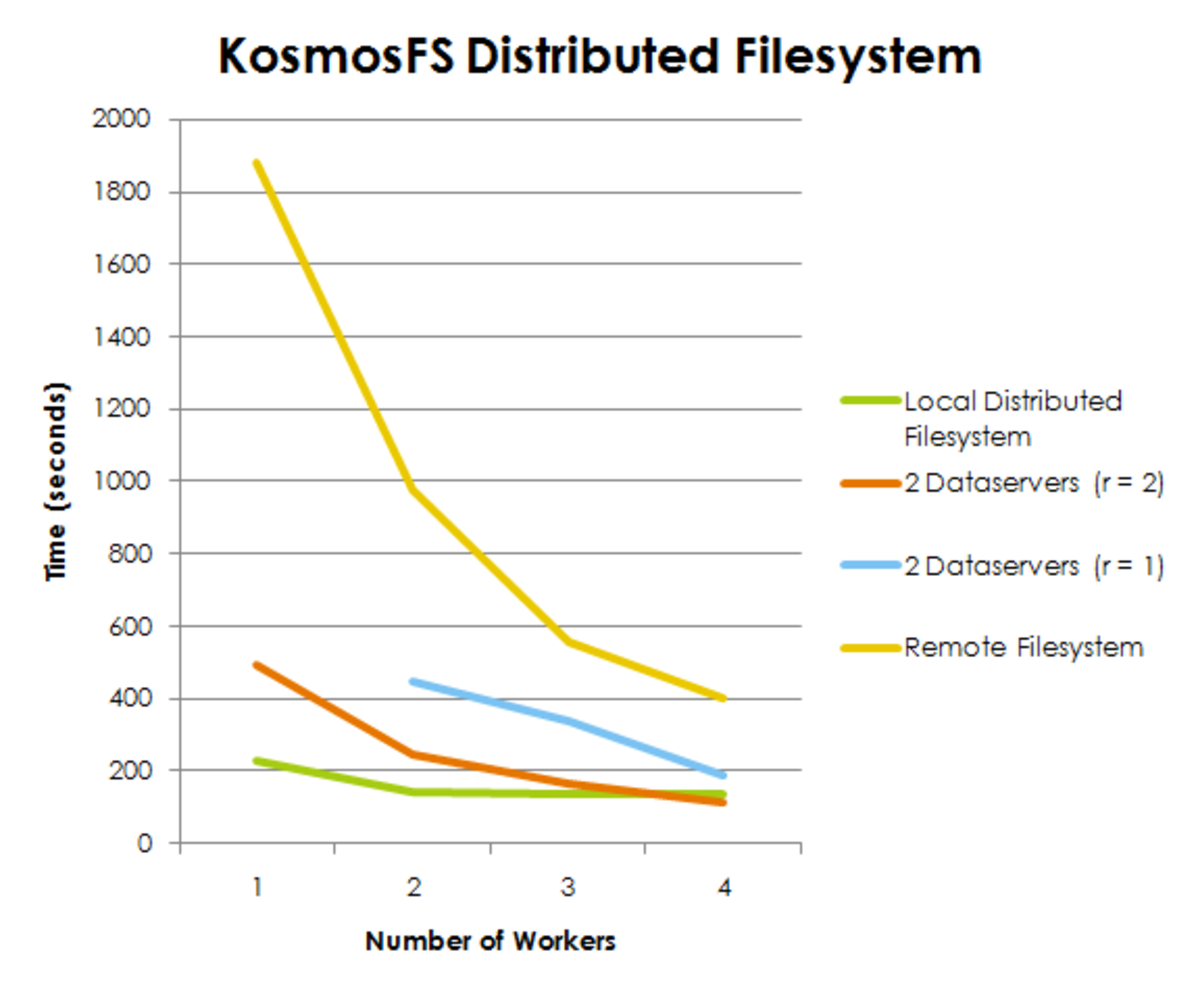
\includegraphics[width=\textwidth]{KFSTest.pdf}
\section{Conclusion}
Our results show that a DFS greatly changes the performance of a
distributed application in a positive manner. Our experiments that
utilised the DFS to access and store data outperformed their gridftp
counterparts by an order of magnitude in most cases. Our results also
indicate that the DFS scales better as file sizes and number of files
grow, although both seem to scale linearly. Before any conclusions may
be drawn, there are issues that need to be addressed. Our application
utilised SAGA to access DFS based and gridftp based files. Although
there is clearly a SAGA induced overhead, this overhead is constant.
\jhanote{ We need to discuss performance issue: Ole has performance
numbers that contradict this, i.e., the overhead that SAGA introduces
for file/gridftp is very small compared to native globus calls. This may
be due to SAGA's adaptive nature, where lots of computation is spent
determining how to make a distributed call. Other reason's may be the
gridftp SAGA adaptor being separated from the application, being able to
make only general decisions, allowing no performance tweaks. }
\jhanote{Accessing files through this abstraction with gridftp seemed to
perform sub-optimally in comparison to using the globus tools directly.}
In addition, we were unable to utilise our entire distributed system,
using at most 8 jobs to handle our work. With a replication level of two
in the DFS, data was almost certainly co-located with the computational
resource. In the second experiment, utilizing information from first
staging the network did improve upon the results of the naive first
experiment, but still did not approach the DFS's performance levels.

Distributed filesystems are important abstractions for a data-intensive
distributed application developers to consider. It also appears that
staging is worth the time required to build a graph representing the
network. Also to note, the second experiment is also naive in the way
that it attempts to optimise data and work assignments. Our staging only
performed pings, not data transfer trials or reliability tests. A job
could have low latency, but poor bandwidth. Perhaps CloudStore's
performance can be attributed to recent work that has shown that data in
large scale distributed applications tends to be accessed together,
despite being seemingly unrelated in the input data-set. Such
correlation in data-access has been observed elsewhere, and specific
abstractions to support the access of ``aggregation of such files'' has
been referred to as a filecule, an application specific group of
files~\citep{filecule}. Attempting to determine if analogous abstractions
could enhance performance for the All-Pair application could be
interesting.  In a DFS, however, if the data store is also capable of
data processing, then the DFS is placing commonly used files together on
machines needing them for work; in essence, the DFS is finding these
groups for the developer. The fault tolerance, for which distributed
filesystems are already well renowned for, also has added benefits to
grid application developers in terms of performance. The distributed
application does not have to be aware of where data has been copied to
previously when assigning work; the distributed filesystem uses the best
replica when data is being accessed.

\fixme{This should be changed to be appropriate \bf{**Shantenu**}}
{\bf Acknowledgment:} This work would not have been possible without the support of 
     the wider SAGA team. Important funding for SAGA
     specification and development has been provided by the UK EPSRC
     grant number GR/D0766171/1 (via OMII).  SJ acknowledges the
     e-Science Institute, Edinburgh for supporting the research theme,
     ``Distributed Programming Abstractions''.  We would also like to
     thank Yaakoub el-Khamra for useful discussions. This work has also
     been made possible thanks to computer resources provided by the
     TeraGrid and LONI.

%\bibliographystyle{IEEEtran}
\bibliographystyle{kluwer} 
\bibliography{data_intensive_paper}
\end{document}
